\begin{center}
  \Large
  \textbf{BIOGRAFI PENULIS}
\end{center}

\addcontentsline{toc}{chapter}{BIOGRAFI PENULIS}

\vspace{2ex}

\begin{wrapfigure}{L}{0.3\textwidth}
  \centering
  \vspace{-3ex}
  % Ubah file gambar berikut dengan file foto dari mahasiswa
  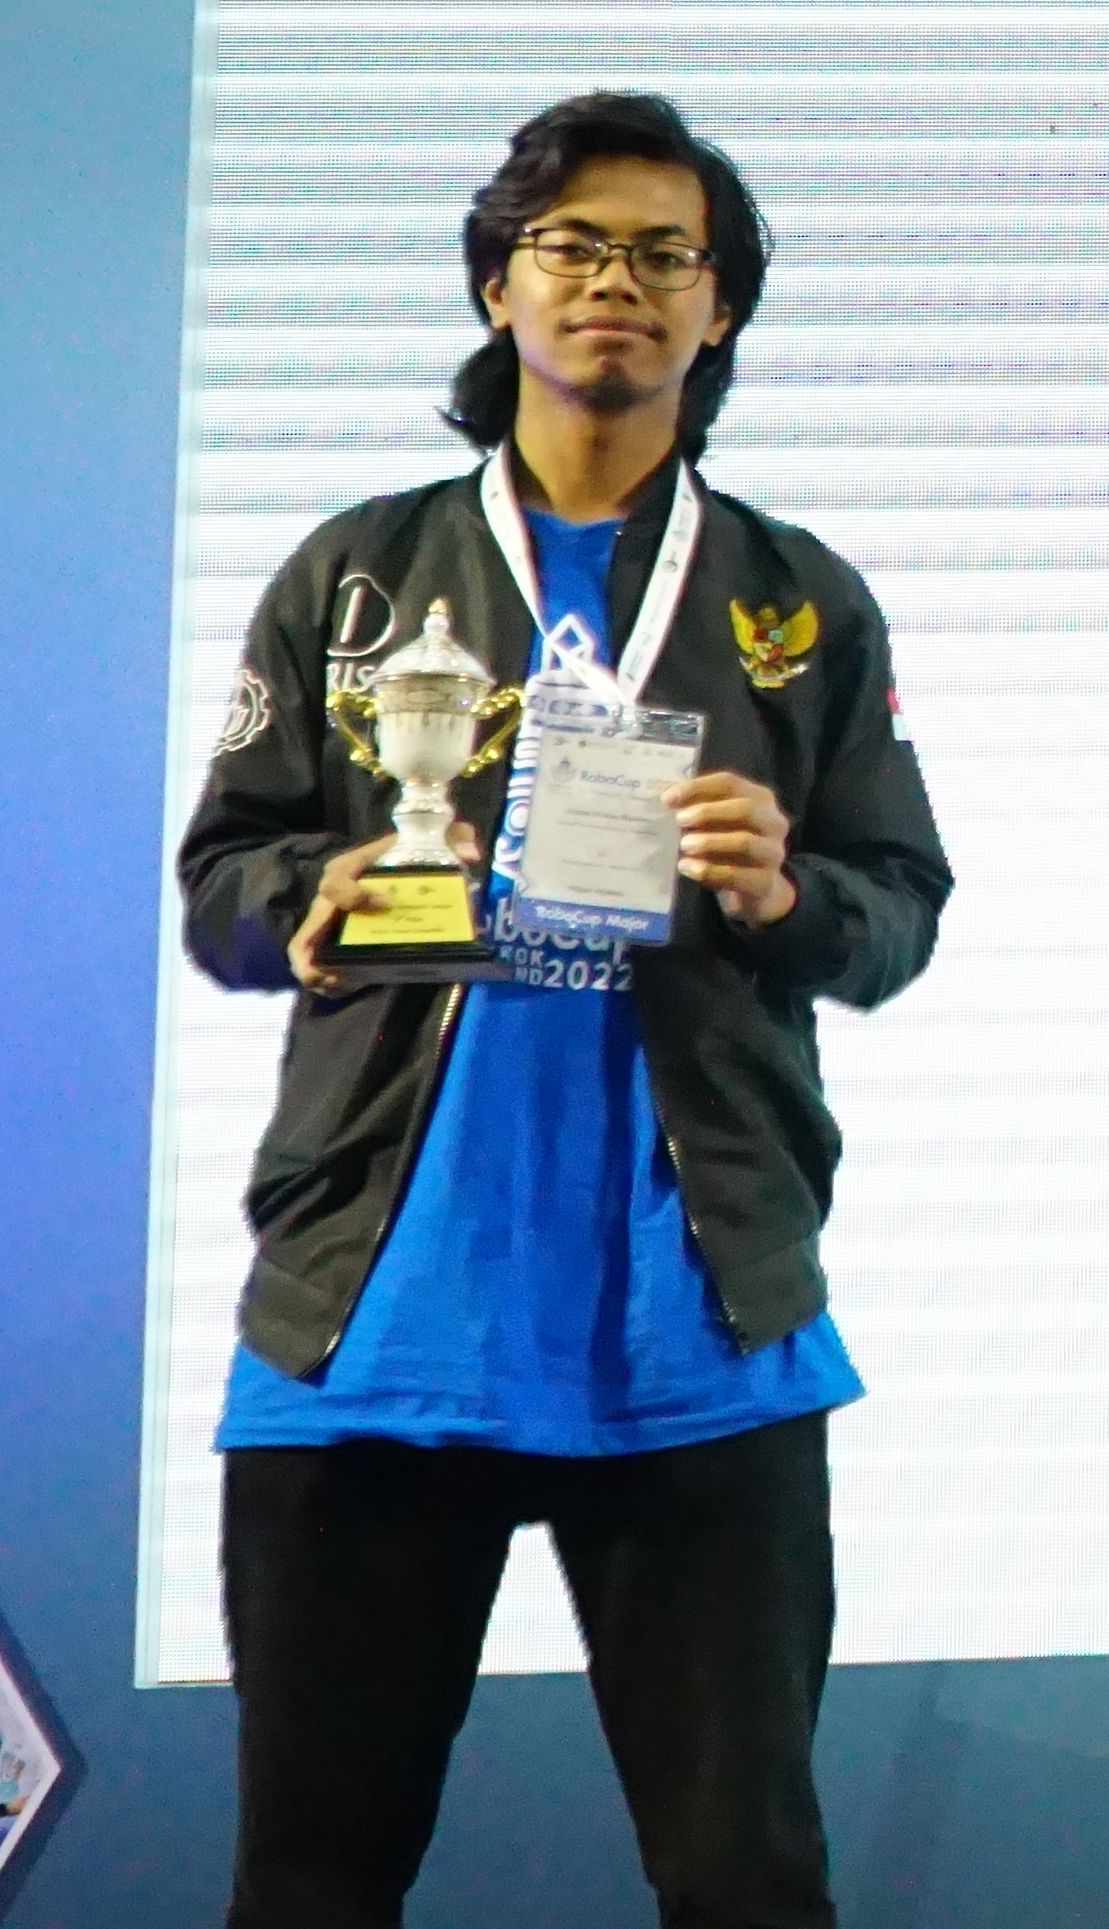
\includegraphics[width=0.3\textwidth]{gambar/foto_piala_asli_cropped.jpg}
  \vspace{-4ex}
\end{wrapfigure}

% Ubah kalimat berikut dengan biografi dari mahasiswa
\name{}, lahir pada 4 Juni 2002, di Jember. Penulis merupakan mahasiswa Program Studi Teknik Komputer angkatan 2020. Penulis aktif dalam kegiatan penelitian dan pengembangan teknologi terutama pada bidang robotika. Penulis juga merupakan programmer utama tim IRIS ITS sejak 2021 yang aktif dalam mengikuti kompetisi robotika baik tingkat Nasional maupun tingkat Internasional. Kejuaraan yang telah diraih penulis antara lain Juara 2 Kontes Robot Indonesia 2021 Regional, Juara 2 Kontes Robot Indonesia 2021 Nasional, juara 2 Robocup Asia Pasific 2021, Juara 1 Kontes Robot Indonesia 2022 Regional, Juara 1 Kontes Robot Indonesia 2022 Nasional, Juara 3 Robocup Internasional yang diselenggarakan di Thailand 2022, Juara 1 Robocup Asia-Pasific 2022, Juara 2 Kontes Robot Indonesia Regional 2023, dan Juara 3 Kontes Robot Indonesia Nasional 2023. Penulis memiliki keyakinan bahwa jika kita berjuang, berusaha, dan berdoa, maka kita akan mendapatkan hasil yang maksimal. Penulis berharap bahwa tugas akhir ini dapat memberikan manfaat bagi pembaca dan dapat menjadi referensi bagi peneliti selanjutnya.